\documentclass[11pt,a4paper]{article}
\usepackage[utf8]{inputenc}
\usepackage{geometry}
\geometry{a4paper, margin=1in}
\usepackage{graphicx}
\usepackage{booktabs}
\usepackage{float}
\usepackage{hyperref}
\usepackage{xcolor}
\usepackage{tcolorbox}
\usepackage{amsmath}
\usepackage{tikz}
\usepackage{listings}
\usepackage{caption}

% Setup colors and listings
\definecolor{codebg}{rgb}{0.95,0.95,0.95}
\definecolor{primary}{HTML}{2B5B84}
\definecolor{accent}{HTML}{E74C3C}

\tcbset{
    commandbox/.style={
        colback=black!85,
        colframe=black!90,
        coltext=white,
        fontupper=\ttfamily,
        boxrule=1pt,
        arc=4pt,
        left=8pt, right=8pt, top=8pt, bottom=8pt
    }
}

\title{\textbf{\Huge FJSP Architecture \& Technical Report}\\ \vspace{0.3cm} \Large Flexible Job-Shop Scheduling Problem Ecosystem}
\author{\textbf{Inter IIT Team}}
\date{\today}

\begin{document}

\maketitle
\tableofcontents
\newpage

\section{Executive Summary}
The Flexible Job-Shop Scheduling Problem (FJSP) is a prominent NP-hard optimization challenge mirroring real-world manufacturing constraints. This technical report details a complete ecosystem encompassing robust instance generation, independent schedule validation, and six distinct heuristic search algorithms.

\textit{Note on Evaluation Scope: While the algorithms have been stress-tested across carefully engineered structural edge cases (bottlenecks, high flexibility, extreme variance), the empirical dataset size remains relatively small ($N=10$ distinct topologies). Consequently, algorithmic superiority claims are formulated contextually rather than as universal absolutes.}

\section{System Architecture}
The ecosystem architecture is designed around strict separation of concerns. Solvers do not parse internal verification structures, and the validator assumes zero trust in solver outputs.

\begin{figure}[H]
    \centering
    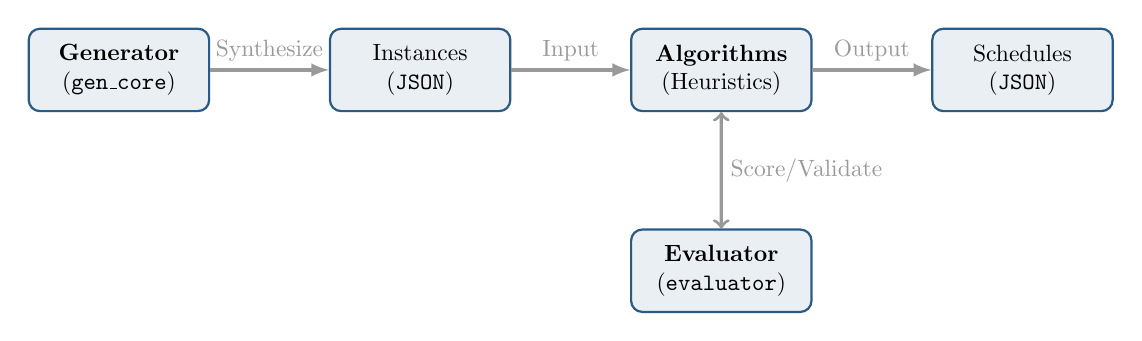
\begin{tikzpicture}[node distance=2cm, auto, thick, scale=0.85, transform shape]
        \tikzstyle{block} = [rectangle, draw=primary, fill=primary!10, text width=7em, text centered, rounded corners, minimum height=3.5em]
        \tikzstyle{line} = [draw, -latex, very thick, color=gray!80]

        \node [block] (gen) {\textbf{Generator} \\ (\texttt{gen\_core})};
        \node [block, right of=gen, node distance=4.5cm] (inst) {Instances \\ (\texttt{JSON})};
        \node [block, right of=inst, node distance=4.5cm] (solver) {\textbf{Algorithms} \\ (Heuristics)};
        \node [block, right of=solver, node distance=4.5cm] (sched) {Schedules \\ (\texttt{JSON})};
        \node [block, below of=solver, node distance=3cm] (eval) {\textbf{Evaluator} \\ (\texttt{evaluator})};

        \path [line] (gen) -- node {Synthesize} (inst);
        \path [line] (inst) -- node {Input} (solver);
        \path [line] (solver) -- node {Output} (sched);
        \path [line, <->] (solver) -- node {Score/Validate} (eval);
    \end{tikzpicture}
    \caption{Modular Data Flow Architecture}
    \label{fig:arch}
\end{figure}

The \textbf{Generator} utilizes stochastic distributions (LogNormal, Gamma) to build robust problem topologies. The \textbf{Algorithms} load these problems and iteratively ping the \textbf{Evaluator} to receive deterministic O(N) scoring.

\vspace{0.5cm}
\begin{tcolorbox}[commandbox, title=Running the Pipeline]
# 1. Synthesize an extreme structural instance
./generator/gen_core.exe --class extreme --jobs 20 --machines 5 --output test.json

# 2. Execute a scheduling algorithm
./algorithms/simulated_annealing.exe --instance test.json --output sched.json
\end{tcolorbox}

\newpage
\section{Algorithm Architecture \& Failure Analysis}

Six scheduling heuristics were implemented. In FJSP, an algorithm must solve two sub-problems simultaneously: \textbf{Machine Assignment (MA)} and \textbf{Operation Sequencing (OS)}. 

\subsection{1. Greedy (Shortest Processing Time)}
\textbf{Architecture:} An iterative, single-pass dispatching heuristic. At each discrete step, it filters topologically available operations and strictly assigns the one yielding the earliest completion time to its fastest machine. \\
\textbf{Complexity:} Space $O(N)$ | Time $O(N^2)$
\begin{itemize}
    \item \textbf{Failure Mode (Bottlenecks):} On the \texttt{low\_flexibility} and \texttt{extreme} configurations, Greedy ECT produced makespans drastically worse than meta-heuristics (e.g., 499 vs 419 on low flexibility).
    \item \textbf{Structural Cause:} Greedy acts with severe short-sightedness. It blindly occupies critical bottleneck machines with low-priority tasks just because they fit momentarily. This blocks operations that \textit{strictly require} that bottleneck, artificially inflating the critical path.
    \item \textbf{Proposed Solution:} \textit{Machine Contention Lookahead.} Weight operations by their flexibility prior to assignment; give strict priority to operations possessing zero alternative routes.
\end{itemize}

\subsection{2. Local Search (LS)}
\textbf{Architecture:} LS seeds an initial Greedy sequence, then stochastically applies neighborhood mutations—either swapping machines in the MA vector or executing topological swaps in the OS vector. \\
\textbf{Complexity:} Space $O(N)$
\begin{itemize}
    \item \textbf{Failure Mode (Stagnation):} On instances with highly isolated global optima (e.g., \texttt{bottleneck}), LS frequently terminates prematurely.
    \item \textbf{Structural Cause:} FJSP search spaces are deeply corrugated. If the topology exhibits a wide local minimum valley, standard LS hits the floor and stagnates entirely, possessing no momentum to escape.
    \item \textbf{Proposed Solution:} Implement Variable Neighborhood Search (VNS) to systematically alter the perturbation strength when stagnation occurs.
\end{itemize}

\subsection{3. Simulated Annealing (SA)}
\textbf{Architecture:} SA acts as a thermodynamic wrapper around Local Search, utilizing a cooling schedule ($T_0=100, \alpha=0.999$) to accept worse solutions probabilistically ($P = e^{-\Delta / T}$). \\
\textbf{Complexity:} Space $O(N)$
\begin{itemize}
    \item \textbf{Failure Mode (Freezing):} While SA dominated the benchmarks (winning 6/10 classes), it exhibited sensitivity to large-scale data ($50 \times 10$).
    \item \textbf{Structural Cause:} A static cooling rate causes the algorithm to freeze too rapidly across massive state spaces, effectively degenerating back into a basic Local Search before the global boundaries are explored.
    \item \textbf{Proposed Solution:} Adaptive reheating. Automatically increase $T$ when the variance of the last 1,000 accepted solutions falls below a threshold.
\end{itemize}

\subsection{4. Tabu Search (TS)}
\textbf{Architecture:} TS maintains a strict memory queue (\textit{Tabu List}) of recently visited states to prevent cycling. Unlike SA, it deterministically evaluates an entire neighborhood array before selecting the best non-Tabu move. \\
\textbf{Complexity:} Space $O(N + L)$ where $L$ is tabu tenure.
\begin{itemize}
    \item \textbf{Failure Mode (Runtime Explosion):} TS performed exceptionally well on \texttt{high\_flexibility} (scoring 147 vs SA's 160) but suffered massive runtime inflation (see Fig \ref{fig:runtime}).
    \item \textbf{Structural Cause:} Evaluating a neighborhood of $K=20$ candidates at \textit{every} iteration requires 20x the evaluator calls of SA.
    \item \textbf{Proposed Solution:} Delta-evaluation techniques. Rather than re-evaluating the entire schedule O(N), calculate only the $\Delta$ change caused by a localized swap.
\end{itemize}

\subsection{5. Genetic Algorithm (GA)}
\textbf{Architecture:} GA maintains a population of schedule arrays, iterating through Job-Based Crossover (JBX) and uniform mutations over successive generations. \\
\textbf{Complexity:} Space $O(P \times N)$ where $P$ is population size.
\begin{itemize}
    \item \textbf{Failure Mode (Structural Destruction):} GA failed completely on the \texttt{large} instance ($50 \times 10$), scoring 434.0 compared to SA's 323.0.
    \item \textbf{Structural Cause:} The FJSP search space scales as $(N!)^M \times M^O$. Random Job-Based Crossover slices the OS vector arbitrarily. In tight FJSP schedules, this violently destroys localized machine packings, producing offspring structurally inferior to both parents.
    \item \textbf{Proposed Solution:} Critical-Path Crossover. Identify the bottleneck sequence in Parent A and strictly preserve it during insertion into Parent B.
\end{itemize}

\subsection{6. Memetic Algorithm (Hybrid GA + LS)}
\textbf{Architecture:} Synthesizes global exploration (GA) with localized exploitation (LS). Every offspring birthed by the GA undergoes a fast, localized descent. \\
\textbf{Complexity:} Space $O(P \times N)$
\begin{itemize}
    \item \textbf{Failure Mode (Efficiency):} While Memetic successfully repaired GA's weaknesses (dropping the \texttt{extreme} makespan from 1130 to 1087 to match SA), it is extremely slow.
    \item \textbf{Structural Cause:} Running a descent algorithm on every individual in a population acts as a massive time multiplier.
    \item \textbf{Proposed Solution:} Partial Memetic strategy. Only apply Local Search to the top 10\% elitist individuals in a generation.
\end{itemize}

\newpage
\section{Experimental Results \& Performance Visualizations}

The benchmarking suite tested these algorithms against hand-crafted topological edge cases. Visualizing these metrics exposes distinct operational trade-offs.

\begin{figure}[H]
    \centering
    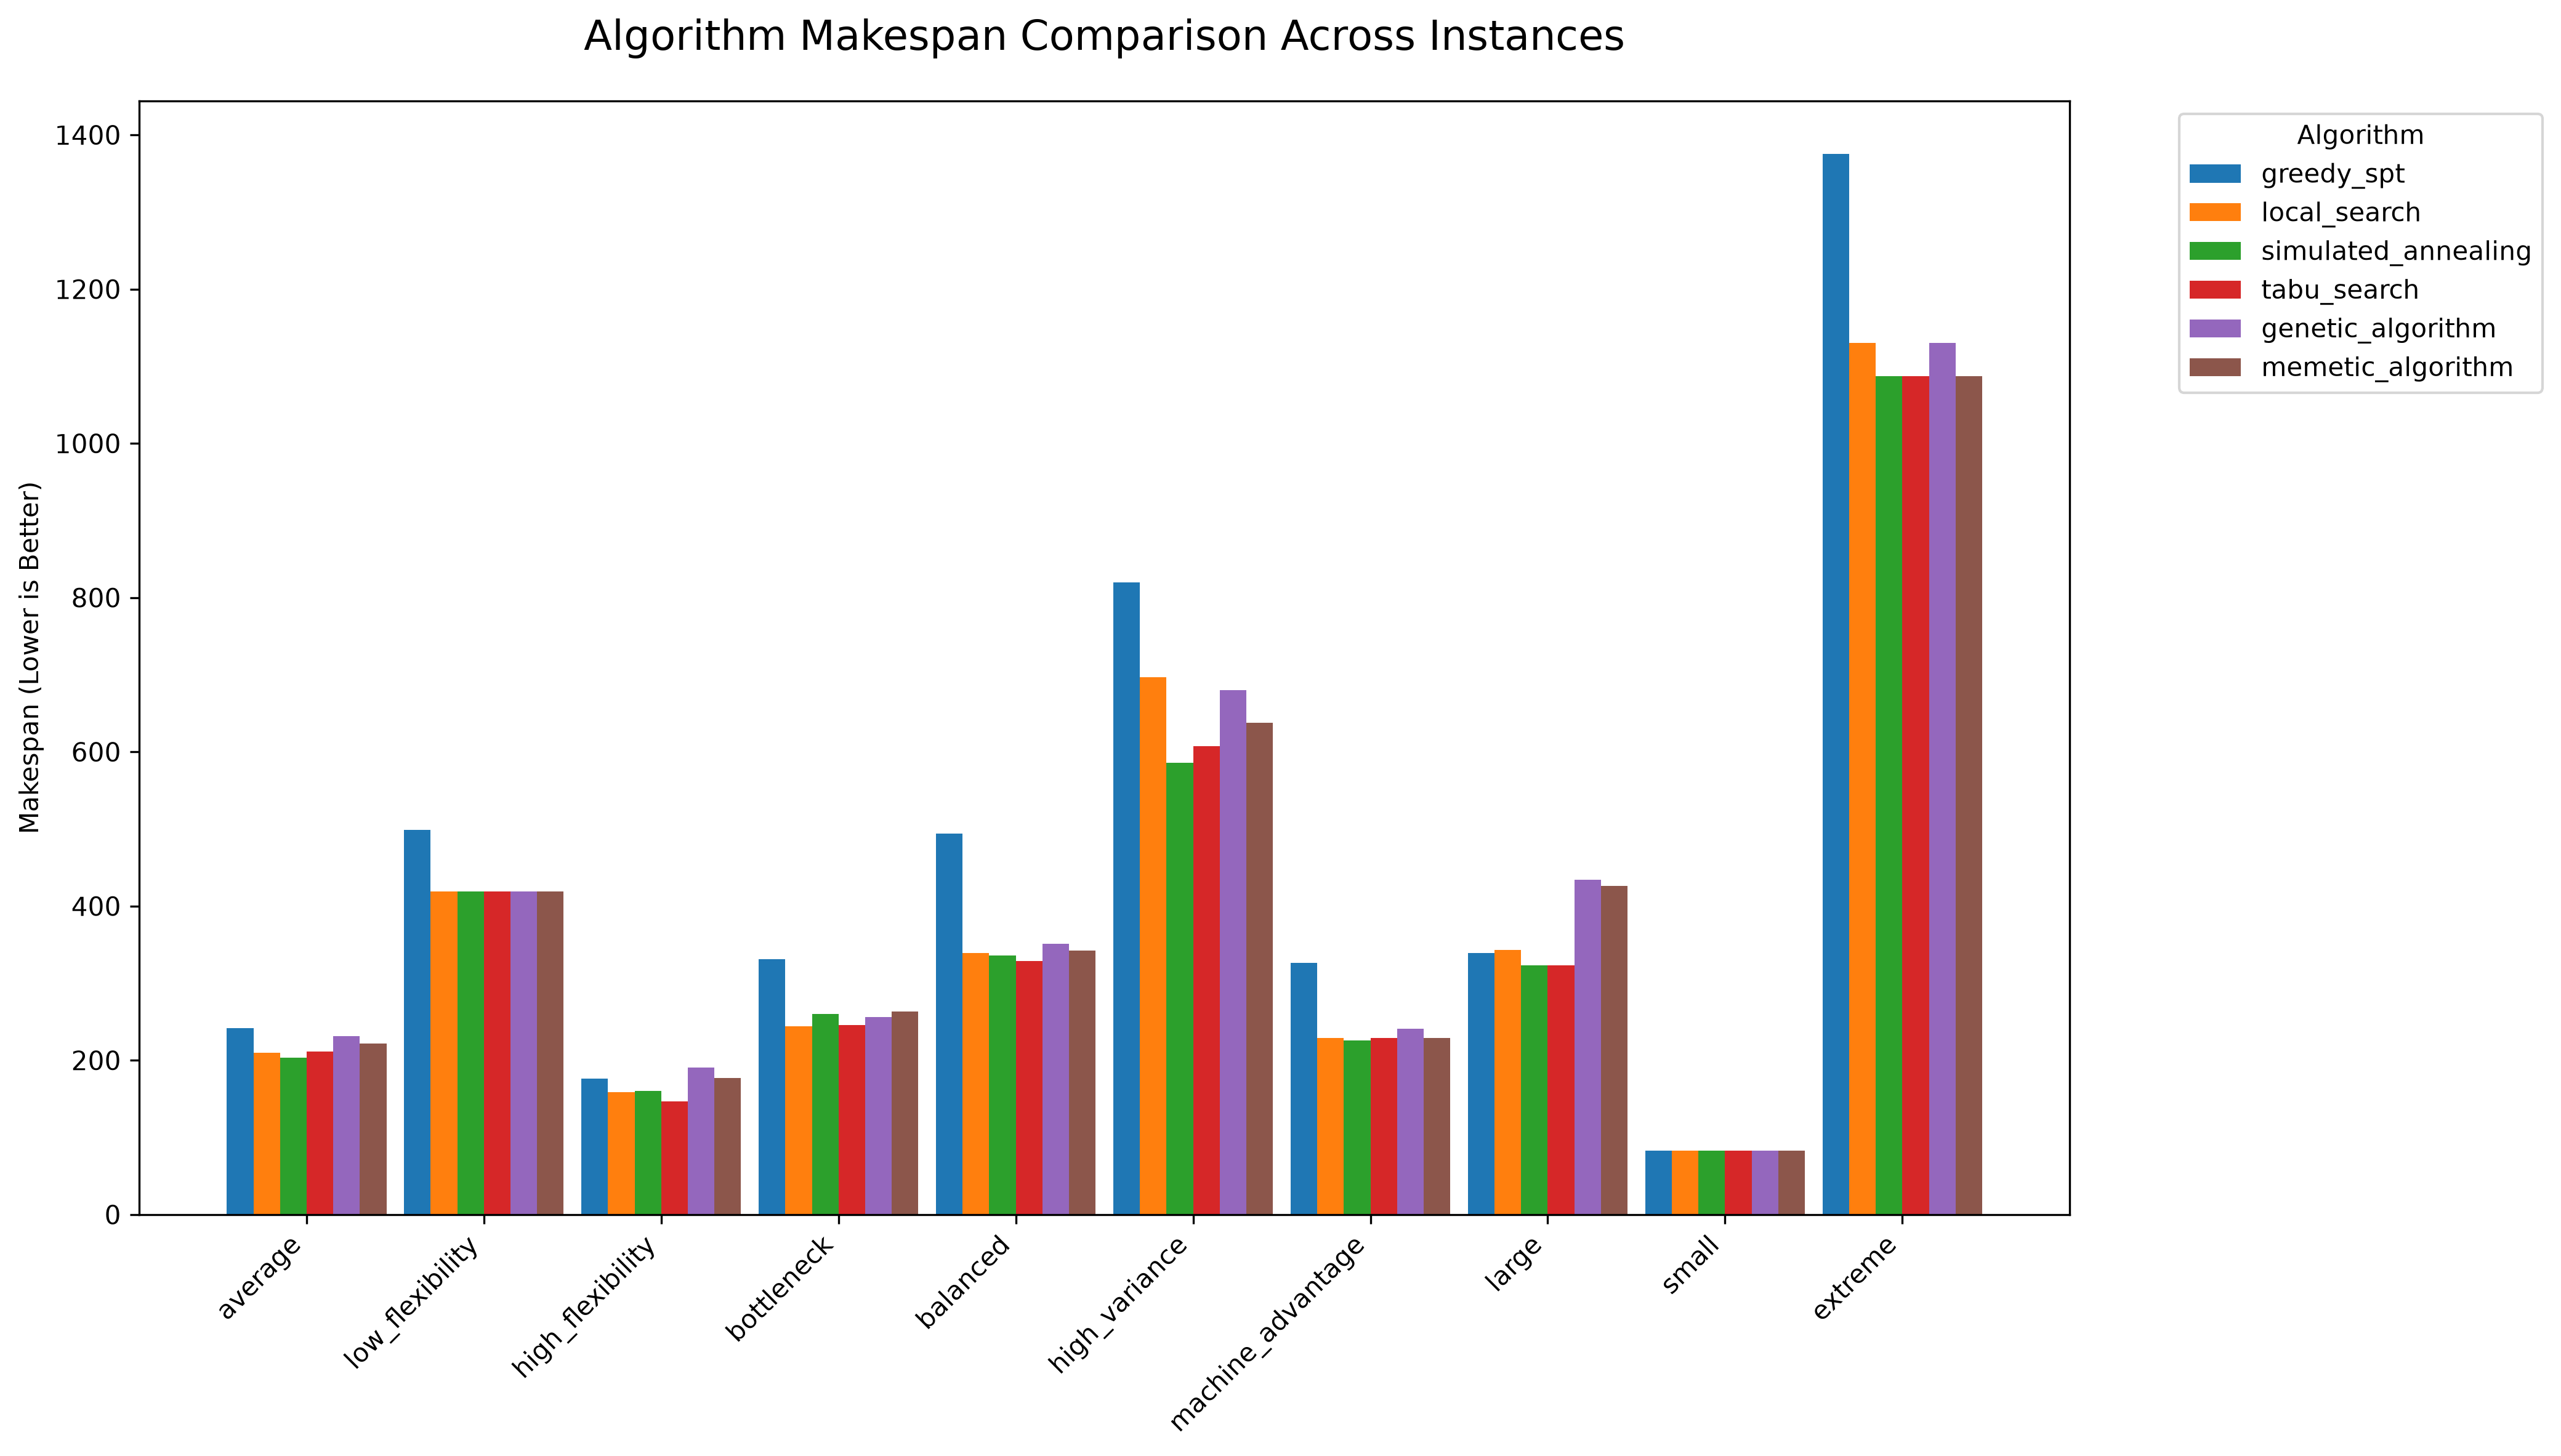
\includegraphics[width=1.0\textwidth]{../analysis/makespan_comparison.png}
    \caption{Algorithm Makespan Comparison. SA and Tabu demonstrate consistent dominance, while Greedy fails under constrained flexibility.}
    \label{fig:makespan}
\end{figure}

\begin{figure}[H]
    \centering
    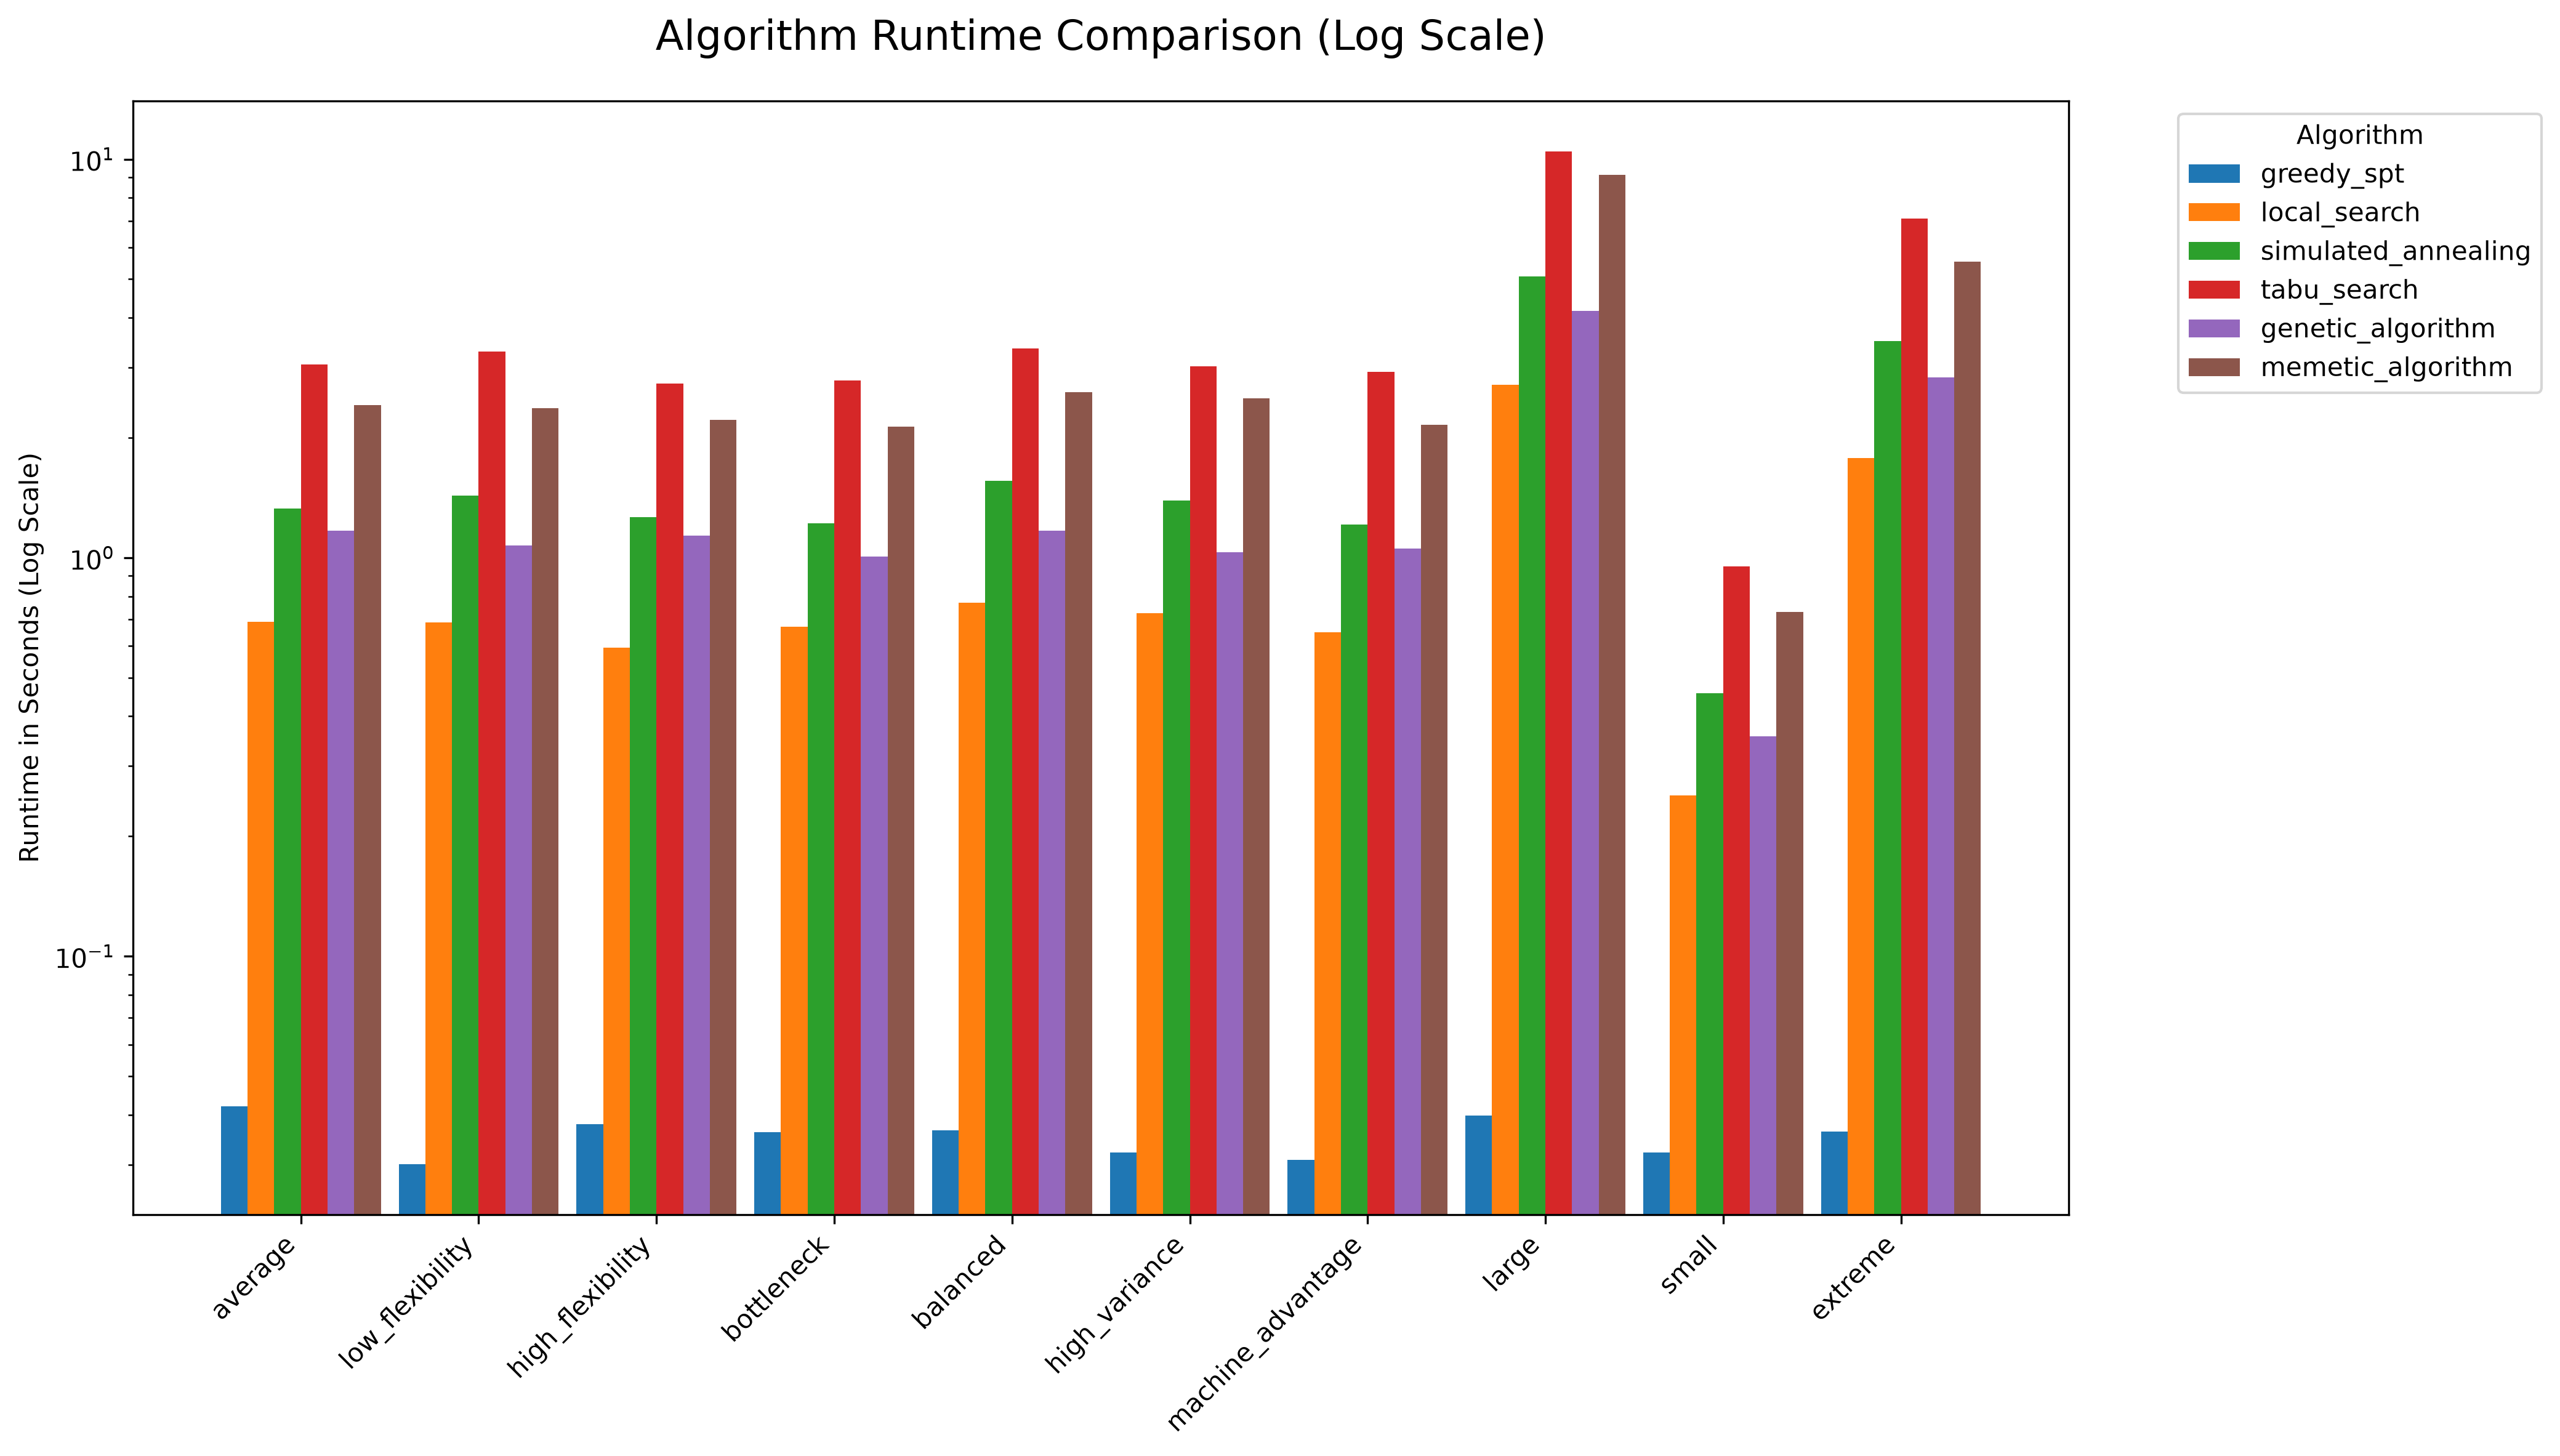
\includegraphics[width=1.0\textwidth]{../analysis/runtime_comparison.png}
    \caption{Log-Scale Runtime Comparison. Notice the immense computational cost of Tabu Search and Memetic Algorithm on large scales compared to SA and Greedy.}
    \label{fig:runtime}
\end{figure}

\subsection{Visualizing Pack Density}
The following Gantt chart visualizes the tight packing achieved by SA, contrasting heavily with the fragmented idle gaps characteristic of Greedy assignments.

\begin{figure}[H]
    \centering
    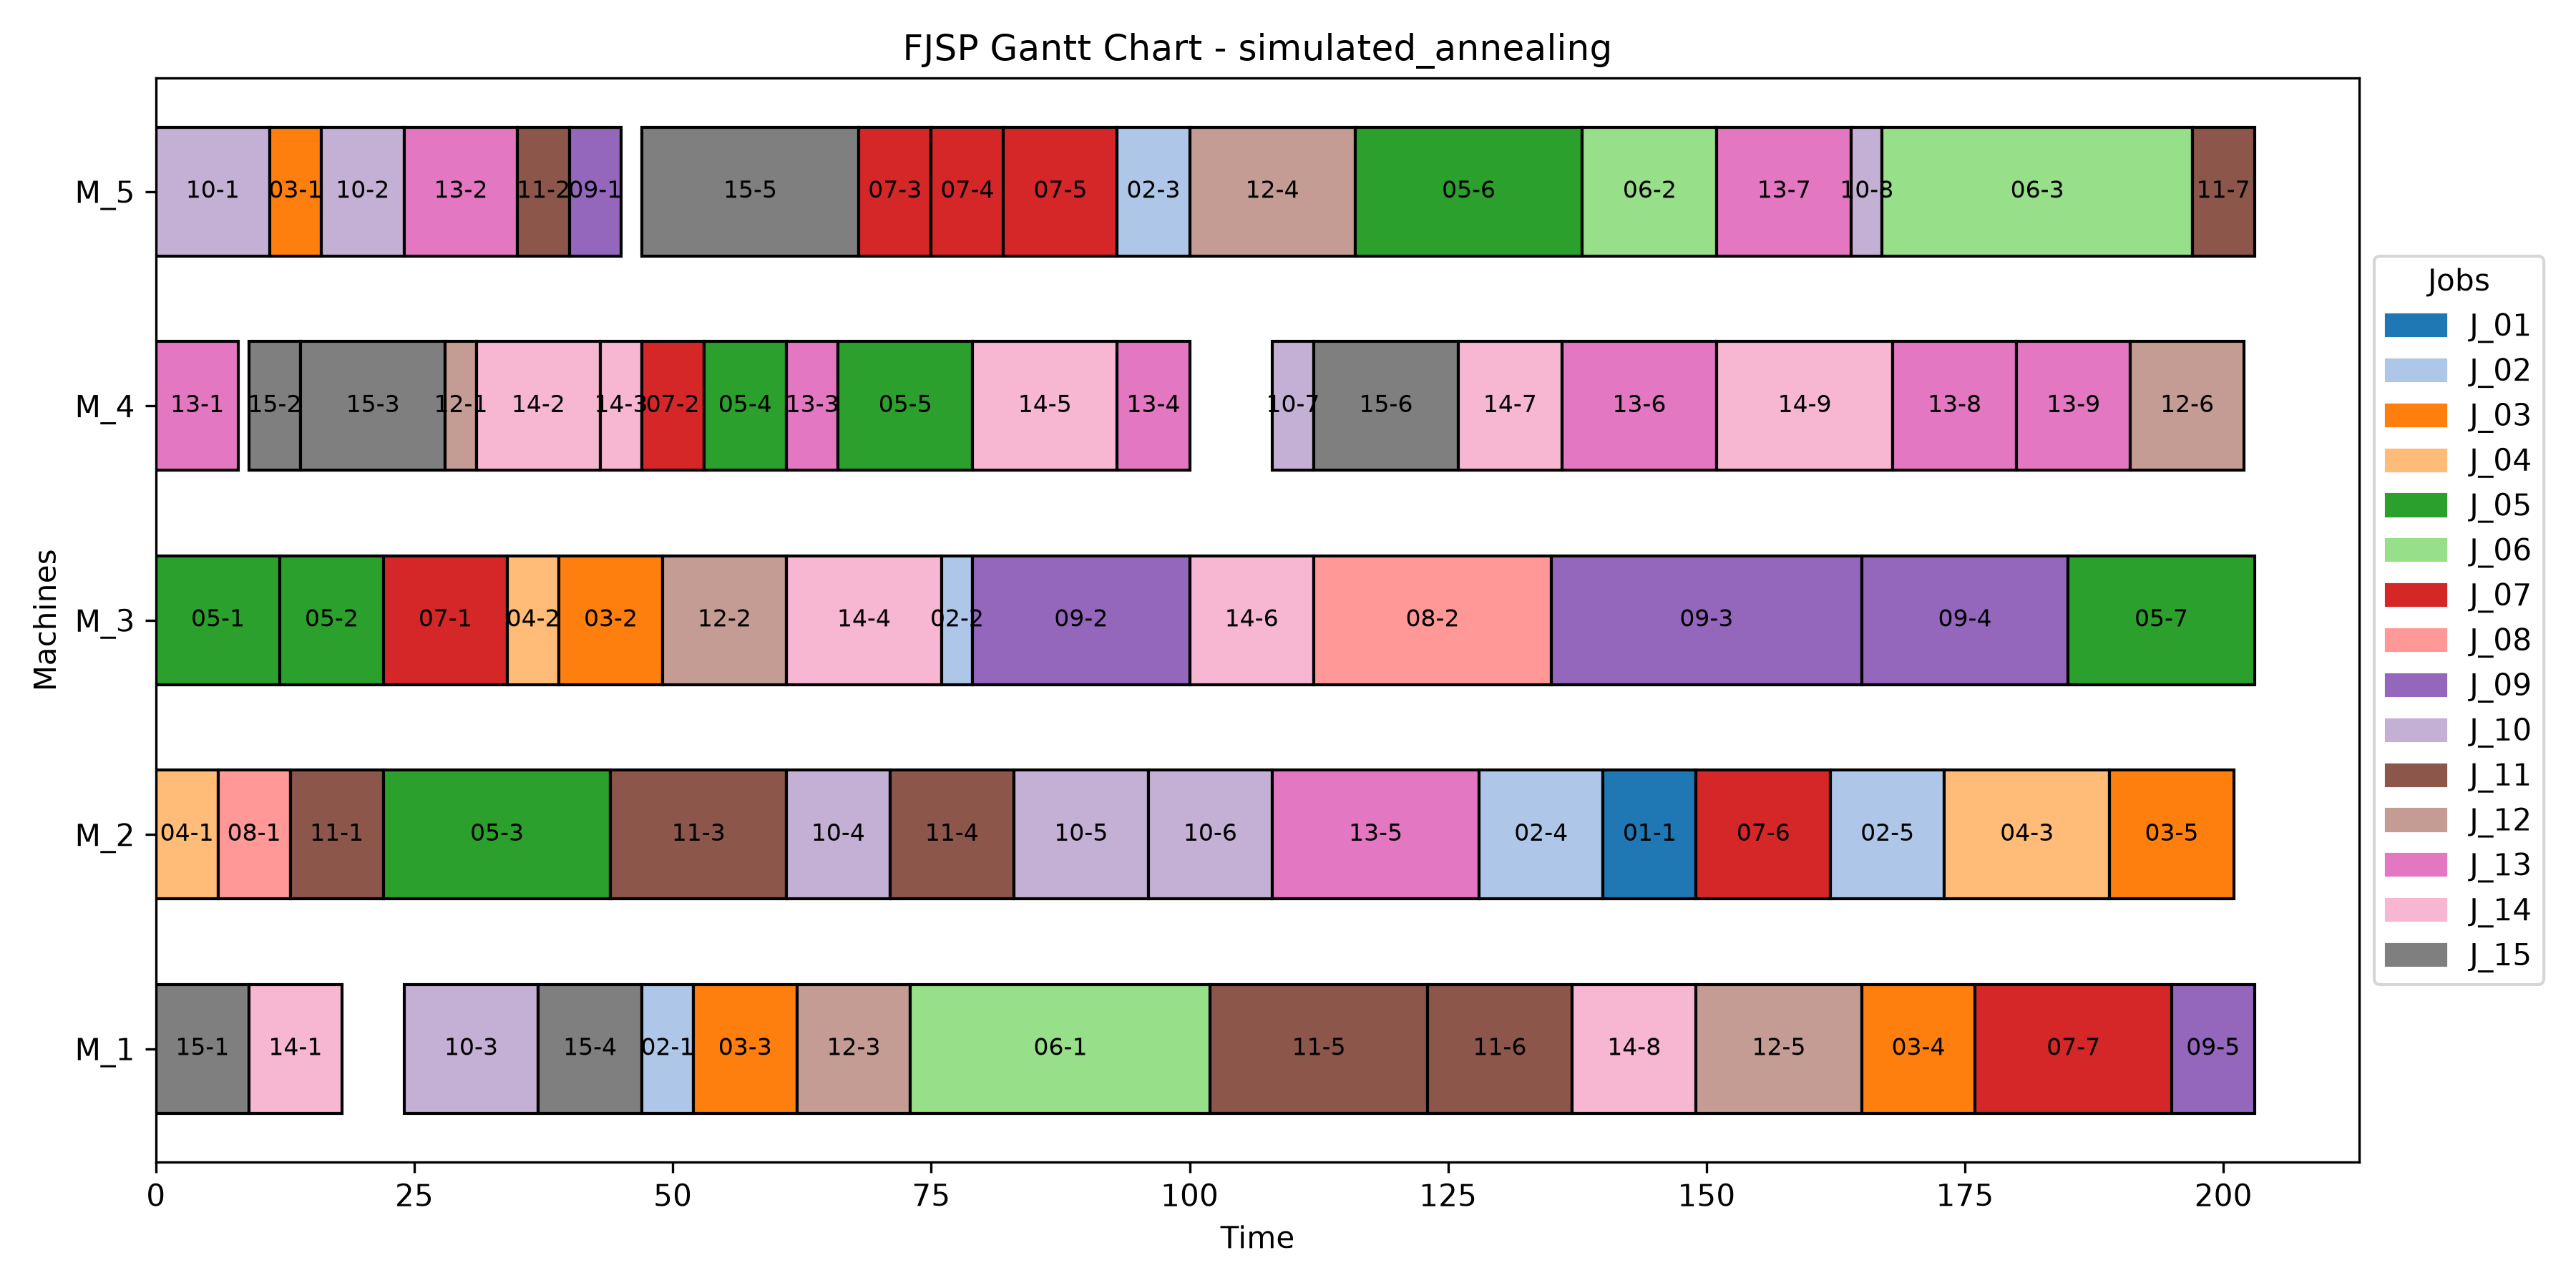
\includegraphics[width=1.0\textwidth]{../analysis/gantt_average_simulated_annealing.png}
    \caption{Gantt Chart (Simulated Annealing on Average Instance). Notice the high density of machine utilization without overlapping conflicts.}
    \label{fig:gantt}
\end{figure}

\section{Conclusion}
This framework succeeds in demonstrating that metaheuristics fundamentally outclass single-pass dispatching rules in constrained flexible environments. Simulated Annealing emerges as the optimal architecture for this domain, providing an unmatched ratio of makespan minimization to computational overhead. However, on strict zero-flexibility constraints (\texttt{low\_flexibility}), all metaheuristics converged identically to the theoretical critical-path floor, proving that mathematical bounds ultimately override algorithmic ingenuity.

\end{document}
